\documentclass[10pt,journal,cspaper,compsoc]{IEEEtran}
%
% If IEEEtran.cls has not been installed into the LaTeX system files,
% manually specify the path to it like:
% \documentclass[12pt,journal,compsoc]{../sty/IEEEtran}

\usepackage{fixltx2e}
% \usepackage{stfloats}
\usepackage{amsmath}
\usepackage{graphicx}
\usepackage{amsfonts}
\usepackage{amsthm}
\usepackage{cite}
\usepackage{algorithm}
\usepackage{algorithmic}
\usepackage{url}
\input{/Users/jovo/Research/latex/latex_commands.tex}
\hyphenation{op-tical net-works semi-conduc-tor}
\newcommand{\Qs}{Q}


\begin{document}

\title{Bayes Optimal Shuffled Graph Classification: Applications in Statistical Connectomics}

\author{Joshua T.~Vogelstein %, Mark Dredze, R.~Jacob~Vogelstein, 
 and 
Carey~E.~Priebe% <-this % stops a space
\IEEEcompsocitemizethanks{\IEEEcompsocthanksitem J.T. Vogelstein and C.E. Priebe are with the Department
of Applied Mathematics and Statistics, Johns Hopkins University, Baltimore, MD 21218.  %\protect\\
% note need leading \protect in front of \\ to get a newline within \thanks as
% \\ is fragile and will error, could use \hfil\break instead.
E-mail: joshuav@jhu.edu
% \IEEEcompsocthanksitem R.J. Vogelstein is with the Johns Hopkins University Applied Physics Laboratory, Laurel, MD, 20723.
}% <-this % stops a space
\thanks{}}
 
% The paper headers
\markboth{IN PREP}%
{Graph Classification}

\IEEEcompsoctitleabstractindextext{%
\begin{abstract}
Graph classification algorithms often do not incorporate vertex label information in their classifiers.  In this work, we investigate the extent to which discarding vertex labels can hinder classification performance, and for which random graph models it would be expected to matter.  Via theory we demonstrate a collection of results.  Specifically, if one ``shuffles'' the graphs prior to classification, the vertex label information is irretrievably lost, which can degrade misclassification performance (and does whenever the vertex labels have class-conditional signal).  Thus, while one cannot hope to recover the labels, trying to recover the labels actually results in a consistent estimate of the optimal graph invariant.  This approach therefore solves the question of ``which invariant to use'' for any graph classification problem, at least asymptotically.  Via simulation we demonstrate that a finite (and small) number of training samples can be sufficient to achieve this bound.  Finally, we apply this approach to a ``connectome'' classification problem (a connectome is the complete set of connections within a brain).  Unshuffling the graphs indeed improves performance, although not over the best performance achievable composing a number of graph invariant and machine learning tools.  Thus, given any unlabeled graph classification problem, the relative performance of an unshuffling approach might be difficult to predict with small sample sizes.
\end{abstract}

% Note that keywords are not normally used for peer review papers.
\begin{keywords}
statistical inference, graph theory, network theory, structural pattern recognition, connectome.
\end{keywords}}


% make the title area
\maketitle
\IEEEdisplaynotcompsoctitleabstractindextext
\IEEEpeerreviewmaketitle



\section{Introduction}

\IEEEPARstart{T}{his} work addresses graph classification in the presence of vertex label shuffling.   
% Consider the following idealized scenario. 
A (labeled) graph $G=(\mc{V},\mc{E})$ consists of a vertex set, $\mc{V}=[n]$, where $n < \infty$ is number of vertices and $[n]=\{1,\ldots, n\}$, and an edge set, $\mc{E} \subseteq [\binom{n}{2}]$.  Vertex labels may or may not be observed.  In the latter case, vertex $v$ in one graph cannot be assumed to correspond to vertex $v$ in another graph.

MOTIVATION


% Graph classification differs from classification of vector-valued random variables in several key aspects.  First, the structure of a graph may encode information.  Second, the vertex labels may or may not be observed.  In unobserved scenarios, NP-hard problems rear their ugly heads \cite{Conte2004}. 


\section{Shuffled-Graph/Class Models} % (fold)
\label{sec:shuffler_graph_class_models}


 Let $\GG: \Omega \mapsto \mc{G}_n$ be a graph-valued random variable taking values $G\in \mc{G}_n$, where $|\mc{G}_n|=2^{\binom{n}{2}}$. 
Let $Y$ be a categorical random variable, $Y: \Omega \mapsto \mc{Y}=\{y_1,\ldots, y_{c}\}$, where $c< \infty$, such that each graph has an associated class.  Assume that graphs and classes are jointly sampled from some distribution, $(\GG,Y) \sim \PP_{\GG,Y}=\PP$.  This joint distribution can be decomposed into the product of a class-conditional distribution (likelihood), $\PP_{\GG|Y}$, and a prior, $\pi_Y$. Because $n$ is finite, the likelihood distributions can be considered discrete distributions, $\PP_{\GG | y}=\text{Discrete}(G; \bth_y)$, for some $\bth_y \in \triangle_d$, where $\triangle_d$ is the $d$-dimensional simplex (that is, $\theta_{i|y}\geq 0$ for all $i \in [d]$ and $\sum_{i \in [d]} \theta_{i|y}=1$, $d=|\mc{G}_n|$). 


In the above, it was implicitly assumed that the vertex labels were observed perfectly.  However, in certain situations, classification performance can improve by relaxing this assumption.  To proceed, we define isomorphic as follows.  Graphs $G,G' \in \mc{G}_n$ are isomorphic to another if and only if there exists a vertex permutation function $\Qs:\mc{G}_n \mapsto \mc{G}_n$ such that $\Qs(G)=G'$.  Let $\QQ$ be a permutation-valued random variable, $\QQ:\Omega \mapsto \mc{Q}_n$, where $\mc{Q}_n$ is the space of vertex permutation functions on $n$ vertices, and $|\mc{Q}_n|=n!$.  Extending the model to include the shuffling distribution yields $\PP_{\QQ,\GG,Y}=\PP'$.  We assume throughout this work (with loss of generality) that the shuffling distribution is both \emph{class independent} and \emph{graph independent}; therefore, this joint model can be decomposed:
\begin{align}
	\PP_{\QQ,\GG,Y} = \PP_{\QQ} \PP_{\GG |Y} \pi_Y.
\end{align}
The shuffled graph distribution can similarly be represented by a discrete distribution: $\PP'_{\QQ(G)|y}(G)=\text{Discrete}(G; \bth_y')$, where $\bth_y' \in \triangle_d$.  When $\PP_{\QQ}$ is uniform, $\bth_y'$  all shuffled graphs within the same isomorphism class are equally likely,  $\{\theta_{i|y}' = \theta_{j|y}' \, \forall i,j$ : $\Qs(G_i)=G_j$ for some $\Qs \in \mc{Q}_n\}$.


An \emph{unlabeled graph} is an isomorphism set: $\mt{G}=\{G: \Qs(G)=G'\}$. Let $\mt{\mc{G}}_n$ be unlabeled graph space. A \emph{shuffle channel}, $\mc{C}: \mc{G}_n \mapsto \mt{\mc{G}}_n$ is a channel that takes as input a graph and outputs an unlabeled graph.  The joint distribution over unlabeled graphs and classes decomposes $\mt{\PP}=\PP{\mt{\GG},Y}=\PP_{\mt{\GG}|Y} \pi_Y$. The class-conditional distributions over isomorphic set (unlabeled graphs) can also be thought of as discrete distributions: $\mt{\PP}_{\GG | y}(\mt{G})=\text{Discrete}(\mt{G}; \eta_y)$, where $\eta_{y}\in \triangle_{\mt{d}}$, and $\mt{d}=|\mt{\mc{G}}_n|$.  Asymptotically, $\mt{d}=d/n!$, with error monotonically decreasing and $>99\%$ accurate for $n>19$ (Ed Scheinerman, personal communication).  Relating $\mb{\eta}_y$ to $\bth_y'$ we have: $\{\theta_{i|y}'=\eta_{j|y}/|\mt{G}_j| \, \forall i : G_i \in \mt{G}_j\}$.  







\section{Bayes Optimal Graph Classifiers} % (fold)
\label{sec:bayes_optimal_graph_classifiers}

% section bayes_optimal_graph_classifiers (end)


A \emph{labeled} graph classifier $h: \mc{G}_n \mapsto \mc{Y}$ is any function that maps from graph space to class space.  The \emph{risk} of a classifier under $0-1$ loss is the expected misclassification rate, $L_{\PP}(h)=\EE_{\PP}[h(G)\neq Y]$.  The optimal classifier is the classifier that minimizes risk:
\begin{align}
	h_*(G) = \argmin_{h \in \mc{H}} \EE_{\PP}[h(\GG) \neq Y].
\end{align}
where $\mc{H}$ is the set of possible classifiers.  Let $L_*=L_{\PP}(h_*)$ indicate minimal (optimal) risk, also called \emph{labeled Bayes risk}.  

A \emph{shuffled} graph classifier $h': \mc{G}_n \mapsto \mc{Y}$ is defined similarly, except it behaves differently by virtue of its input being a shuffled graph, not a labeled graph, so it should somehow ``unshuffle'' prior to classifying, to the extent possible.  Under $0-1$ loss, the \emph{shuffled Bayes risk}, $L'_*=L_{\PP'}(h'_*)$ is the risk of the shuffled Bayes classifier:
\begin{align}
	h_*'(G') = \argmin_{h \in \mc{H}} \EE_{\PP'}[h'(\GG') \neq Y].
\end{align}

An \emph{unlabeled} graph classifier $\mt{h}: \mt{\mc{G}}_n \mapsto \mc{Y}$ is any function that maps from unlabeled graph space to class space.  The \emph{unlabeled Bayes risk}, $\mt{L}_*=L_{\mt{\PP}}(\mt{h}_*)$ is the risk of the unlabeled Bayes classifier:
\begin{align} \label{eq:unbayes}
	 \mt{h}_*(\mt{G}) = \argmax_{y \in \mc{Y}} \EE_{\mt{\PP}}[\mt{h}(\mt{\GG}) \neq Y].
\end{align}

The above three classifiers can be written explicitly in terms of their model parameters:
\begin{align}
	h_*(G) &= \theta_{G|y}\pi_y \\
	h_*'(G') &= \theta_{G'|y}' \pi_y \\
	\mt{h}_*(\mt{G}) &= \eta_{\mt{G}|y}\pi_y
\end{align}


% 
% 
% 
% 
% 
% \section{Model Based Graph Classifiers} % (fold)
% \label{sec:model_based_graph_classifiers}
% 
% % section model_based_graph_classifiers (end)
% 
% % Let $\PP=\PP_{\GG,Y}$ indicate a joint distribution of graphs and classes. 
% The joint distribution over graphs and classes may be decomposed into the product of a likelihood and prior term: $\PP_{\GG,Y} = \PP_{\GG|Y}\pi_Y$, where $\PP_{\GG | Y }$ denotes the class-conditional distribution (likelihood), and 
%  $\pi_Y$ denotes class prior probabilities.
% 
% % $P[Y=y]\overset{\triangle}{=}P[\{\omega: Y(\omega)=y\}]$, 
% % and let .  
% % Assuming the data were sampled from a distribution, $\PP_{\GG,Y}$, a 
% A Bayes optimal graph classifier chooses the maximum a posteriori class \cite{DEV96}:
% \begin{align} \label{eq:bayes}
% 	 h_*(G) = \argmax_{y \in \mc{Y}} \PP_{\GG | y}(G) \pi_{y},
% \end{align}
% where $\PP_{\GG|y}=\PP_{\GG|Y=y}$ and $\pi_y=\pi_{Y=y}$. Let $\mt{\PP}=\PP_{\mt{\GG},Y}$ indicate the joint distribution of unlabeled (or shuffled) graphs and classes.  In other words, $\mt{\PP}$ is the same as $\PP$ except that the graphs have been passed through a shuffle channel, so $\PP$ is a distribution over graphs, and $\mt{\PP}$ is a distribution over sets of isomorphic graphs.  A Bayes optimal unlabeled graph classifier is:
% 
% A Bayes optimal shuffled graph classifier:
% \begin{align}
% 	h'_*(G)=\argmax_{y\in\mc{Y}}\PP_{\GG|y}(G)\pi_y,
% \end{align}
% which is independent of the shuffling distribution.
% 
% Let $L_*$, $\mt{L}_*$, and $L'_*$ be the Bayes risk, unlabeled Bayes risk, and shuffled Bayes risk under $\PP$, $\mt{\PP}$, and $\PP'$, respectively.  

For brevity, we will use the shorthand $\PP_y=\PP_{\GG | Y = y}$, $\mt{\PP}_y=\PP_{\mt{\GG} | Y = y}$ and $\PP'_y=\PP_{\GG|Y=y}'$. 





% \section{Results} % (fold)
% \label{sec:results}

\section{Shuffling Can Degrade Optimal Performance} % (fold)
\label{sec:shuffle}

% subsection pre_and_post_shuffled_bayes_optimal_performance (end)
The result of passing a graph through a shuffle channel can only degrade, but not improve Bayes risk.  This is a restatement of the data processing lemma for this scenario. Specifically, \cite{DEV96} shows that the data processing lemma indicates that in the classification domain, $L^*_X \leq L^*_{T(X)}$, for any statistic $T$ and data $X$.  In our setting, this becomes:

\begin{thm} \label{thm:1}
$L_* \leq \mt{L}_*=L_*'$.
\end{thm}

\begin{proof}
	Assume $|\mc{Y}|=2$ and $\pi_0=\pi_1=1/2$.  
\begin{align} \label{eq:thm1}
	\mt{L}_*&=\sum_{\mt{G} \in \mt{\mc{G}}_n} \min_y \mt{\PP}_{y}(\mt{G})
	% \nonumber \\&
	=\sum_{\mt{G} \in \mt{\mc{G}}_n} \min_y \sum_{G' \in \mt{G}}\PP_y(G')
	\nonumber \\& \geq \sum_{\mt{G} \in \mt{\mc{G}}_n}\sum_{G' \in \mt{G}}\min_y\PP_y(G')=L_*.
\end{align}
It is trivially true that $\mt{L}_*=L_*'$.
\end{proof}



An immediate consequence of the above proof is that the inequality in Theorem \ref{thm:1} is a \emph{strict inequality} whenever the inequality in Eq. \ref{eq:thm1} is strict:

\begin{thm}
	$L_* < \mt{L}_*$ whenever $$\min_y \mt{\PP}_{y}(\mt{G}) > \sum_{G' \in \mt{G}}\min_y\PP_y(G')$$.
\end{thm}

A corollary of the above theorem is that even when the labels \emph{do} carry some class-conditional signal, it may be the case that a shuffle channel does not degrade performance.  In other words, to state that labels contain information is equivalent to stating that some graphs within an isomorphism class are class-conditionally more likely than others: $\exists \, \theta_{i|y} \neq \theta_{j|y}$ and $\Qs(G_i)=G_j$ for some $G_i,G_j \in \mc{G}_n$ and $\Qs \in \mc{Q}_n$, and that $\theta_{i|y}\neq \theta_{i|y'}$ or $\theta_{j|y}\neq \theta_{j|y'}$.  Shuffling has the effect of ``flattening'' likelihoods within isomorphism classes, $\Qs(\bth_y)=\bth_y'$ where $\bth'$ satisfies $\{\theta_{i|y}'=\eta_{j|y}/|\mt{G}_j| \, \forall i : G_i \in \mt{G}_j\}$.  But just because the shuffling changes class-conditional likelihoods does \emph{not} mean that Bayes risk must also change.


This surprising (to us) result follows immediately upon realizing that posteriors can changes without classification performance changing.  The above results hold in the absence of equal priors, and are easily generalized to  $n$-class classification problems.  To see that, simply replace each minimum with a sum over all non-maxima: $$\min_y \PP_y(G) \mapsto \sum_{y \in \mc{Y}'} \PP_y(G) \text{ where } \mc{Y}' =\{y : y \neq \argmax_y \PP_y\}.$$



\section{Bayes Optimal Graph Invariant-Based Classification After Shuffling} % (fold)
\label{sec:gi}

A graph invariant is any function: $\psi: \mc{G}_n \mapsto \Real^{d'}$  for some $d' < \infty$ such that $\psi(G)=\psi(\Qs(G))$ for all $G \in \mc{G}_n$ and $\Qs \in \mc{Q}_n$.  A graph invariant based classifier, $h^{\psi}$ first projects a graph into an invariant space and then classifies.  The Bayes optimal graph invariant classifier minimizes risk over all invariants: 
\begin{align}
	h_*^{\psi}=\argmin_{\psi \in \Psi, h^{\psi} \in \mc{H}^{\psi}} \EE_{\PP'}[h^{\psi}(\GG)\neq Y],
\end{align}
where $\Psi$ is the space of all possible invariants and $\mc{H}^{\psi}$ is the space of classifiers using invariant $\psi$.   $L_*^{\psi}$ is the Bayes invariant risk.  (NOTE TO CEP: I'm not sure that the above expectation is with respect to $\PP'$, though it seems like it must be?)

\begin{thm}
	$\mt{L}_*=L_*^\psi$.
\end{thm}

\begin{proof}
 Let $f_{G'}(G)$ be a graph matching function, that is, $f: \mc{G}_n \times \mc{G}_n \mapsto \{0,1\}$, taking value unity whenever $G$ and $G'$ are isomorphic to one another.  Let $\psi(G)=\mb{f}(G)$, where $\mb{f}=(f_{G_1}, \ldots, f_{G_{\mt{d}}})$.  In words, $\phi(G)$ outputs a vector of length $\mt{d}$ with a single non-zero entry in the isomorphism class of $G$.  Let $h^{\psi}$ be an indicator function for the maximum a posteriori class of the corresponding isomorphism class. For instance, if $G \in \mt{G}_j$, then
\begin{align}
	h^{\psi}= \argmax_{y \in \mc{Y}} \eta_{j|y} \pi_y.
\end{align}
Thus, this graph invariant based classifier is the Bayes unlabeled graph classifier.
\end{proof}



\section{A consistent and efficient unshuffling-based classifier} % (fold)
\label{sec:bayes_optimal_graph_invariant_based_classifier}


thm 4: use carey's f, prove consistency, because things are finite, law of large numbers.  Since all estimates are of discrete probabilities, and there are a finite number of them, the law of large numbers implies convergence.


Section \ref{sec:shuffle} shows that one cannot fruitfully ``unshuffle'' graphs: once they have been shuffled by a uniform shuffler, the label information is lost.  Section \ref{sec:gi} shows that if graphs have been uniformly shuffled, there is a relatively straightforward algorithm for optimally classifying. However, that classifier depends on knowing $\PP'$ a priori, a (typically) poor assumption. Instead of assume that we have $\PP'$, we make a somewhat more reasonable assumption that a collection of data exists, $\{(\QQ_i,\GG_i,Y_i)\}_{i \in [s]}$, and each datum was independently sampled from the same distribution, $(\QQ_i,\GG_i,Y_i)\overset{iid}{\sim}\PP'$.  Sadly, we only observe some \emph{training data} $\mc{T}_s=\{\GG_i',Y_i\}_{i \in [s]}$, where $\GG_i'=\QQ_i(\GG_i)$, and are thusly unable to observe the vertex labels.  Moreover, $\PP_{\QQ}$ is uniform, such that all label information is both unavailable and irrecoverable.  Our task is to induce a classifier, $\mh{h}_s: \mc{G}_n \times (\mc{G}_n \times \mc{Y})^s \mapsto \mc{Y}$ that approximates $\mt{h}_*$ as closely as possible by utilizing the training data.  

A Bayes plugin unlabeled graph-classifier estimates the likelihood and prior terms and plugs them in to Eq. \eqref{eq:unbayes}
\begin{align} \label{eq:class}
	\mh{h}_s(G)=\argmax_{y\in\mc{Y}} \mh{\PP}_{\mt{\GG}|Y=y}(G)\mh{\pi}_y
\end{align}

\begin{thm} \label{thm:conv}
	$\mh{h}_s \conv \mt{h}^*$ as $s \conv \infty$
\end{thm}

\begin{proof}
Given consistent estimators for $\mt{\PP}_y(G)$ and $\pi_Y$, the Bayes plugin classifier is also consistent \cite{DEV96}.  Formally, if $\mh{\PP}_y(G) \conv \PP_y(G)$ and $\mh{\pi}_Y\conv \pi_Y$ as $s \conv \infty$, then $\mh{h}_s \conv \mt{h}_*$ as $s\conv \infty$.  Because $\mc{G}_n$ and $\mc{Y}$ are both finite, the empirical histograms, $\{\mh{\PP}_{\mt{G}|y}\}_{y\in \mc{Y}}$ and $\mh{\mb{\pi}}=(\mh{\pi}_{y_0},\ldots, \mh{\pi}_{y_{c}})$, are guaranteed to converge to the true histograms by law of large numbers.  Thus, $\mh{h}_s \conv \mt{h}^*$ as $s \conv \infty$.
\end{proof}


% As described above, the class-conditional distributions of unlabeled graphs can be characterized as  categorical distributions, $\PP_{\mt{\GG}|Y=y}=\text{Cat}(\mb{\eta}_y)$.  Because a categorical distribution is in the exponential family, the maximum likelihood estimate for its parameters are exist, are unique, consistent, and efficient.  Moreover, the class prior can also be represented as a categorical random-variable, and therefore has the same properties.  Taken together, these results demonstrate that the Bayes plugin unlabeled graph classifier is consistent and efficient.

\section{A Practical Approach to Unlabeled Graph Classification} % (fold)
\label{sec:a_practical_approach_to_unlabeled_graph_classification}

Although Eq. \ref{eq:class} yields consistency from Theorem \ref{thm:conv}, however, utilizing this is practically hopeless.  In the unlabeled case, this requires solving an infinite number of NP-hard problems.  Specifically, using Eq. \ref{eq:conv} requires $\mb{f}$ from Section \ref{sec:gi}, which is a graph matching function.  Graph matching is known to be NP-hard \cite{Conte04}.  Although there is some hope because most graph matching problems can be solved in polynomial time \cite{Conte04}, that hope is lost upon discovering that the constant is crazy large \cite{Conte04}.  We therefore consider an approximate approach as follows.

We assume $(\QQ,\GG,Y), (\QQ_1,\GG_1,Y_1),\ldots, (\QQ_s,\GG_s,Y_s) \overset{iid}{\sim} \PP'$, and we only observe $\GG', \mc{T}_s$, where  $\mc{T}_s=\{(\GG_i',Y_i)\}_{i \in [s]}$ and $\GG_i'=\QQ_i(\GG_i)$. Given these training data $\mc{T}_s$, we proceed as follows.  

For each class, $y \in \mc{Y}$, choose an exemplar (or prototype \cite{Bunke2011}) shuffled graph, $\GG'_{y+} \in \{\GG_i'\}_{i: y_i=y}$.  Then, try to ``unshuffle'' each shuffled graph in each class to its corresponding prototype using an inexact graph matching algorithm, $\mh{f}_y=\mh{f}_{\GG'_{y+}}$.  Although many inexact graph matching algorithms are available, we select the quadratic assignment problem (QAP) based approach developed in \cite{VP11QAP}, which is cubic in $n$ and outperforms the previous state-of-the-art on all benchmarks tested.  This yields $\{\mh{\GG}_i\}$, which we can then use to estimate the \emph{labeled} likelihoods, $\PP_{\GG|Y=y}$.   

Now, although it may seem as we projected our graphs from a space of cardinality $\mt{d}$ to $\mt{d} \times n!$, given the labeled graphs, a variety of asymptotically optimal graph classification algorithms are available with much faster convergence rates (under much simpler models).  Specifically, we choose to use the signal-subgraph classifier developed in \cite{VP11sigsub}.  Under the independent edge assumption, the likelihood of an edge is given by $\PP[A_{uv}|Y=y]=\PP_{uv|y}$, yielding a likelihood factorization: $\PP_y=\prod_{uv}\PP_{uv|y}$. Thus, the class-conditional distribution is given by a matrix, $P_y \in (0,1)^{n \times n}$.   The labeled graphs, $\{\mh{\GG}_i\}$ can be used to estimate these likelihood matrices, $\{P_y\}$, as described in \cite{VP11sigsub} using L-estimators to bound the estimates from the boundaries.   Now, we can use a Bayes plugin labeled graph classifier via the class-conditional posterior estimates:
\begin{align}
	\mh{y}=\argmax_{y \in \mc{Y}} \mh{\rho}_y 
	\text{ where } \mh{\rho}_y=\mh{\PP}_{uv|y}(\mh{f}_y(G)) \mh{\pi}_y.
\end{align}


To gain some intuition with regard to why this approach would be successful, consider the following simple yet illustrative example.  Let each $\mt{\PP}_y$ puts all its mass on a single but distinct isomorphism class, so $\eta_{j|y_j}=1$ and $\eta_{j'|y_j}=0 \, \forall j' \neq j$.  Thus, if $\mh{f}_y$ worked, then every edge present in a class would have unity likelihood, and all other edges would have zero likelihood.  Thus, a single class will have a posterior estimate equal to unity, which will therefore be the maximum a posteriori class.  This simple example can be extended without modification
to allow each class have a non-overlapping set of non-zero likelihoods.  Moreover, reverting to the simple two-class and two non-zero likelihood scenario, consider a different generalization.  %Let both classes have the same two non-zero likelihood values, that is $\eta_{i|y_i} > 0$ for $i=0,1$.  But, let the likelihoods be highly unbalanced, such that $\eta_{0|y_0} /gg \eta_{1|y_0}$ and $\eta_{1|y_1} \gg \eta_{0|y_1}$.  In class 1, the independent edge model would have zeros in all edges that are not in either class under some prototype choice.  


% section a_practical_approach_to_unlabeled_graph_classification (end)


% section bayes_optimal_graph_invariant_based_classifier (end)

\section{Simulated Experiment} % (fold)
\label{sec:simulated_experiment}

To demonstrate the practically of an isomorphism-based unlabeled graph classifier, we conduct the following simulated experiment. Sample $s+1$ triplets identically and independently from the joint shuffler/graph/class model, $(\QQ_i,\GG_i,Y_i)\overset{iid}{=}\PP'=\PP_{\QQ}\PP_{\GG|Y} \pi_Y$, where $\PP_{\QQ}$ is uniform, and $\pi_Y$ is Bernoulli so $\pi_0=\pi_1=1/2$.  The edges are independent so the likelihood factorizes as above.  Specifically, we let $\PP_{uv|0}=$Bernoulli$(p_{uv|y})$, where $p_{uv|0} \overset{indep.}{\sim}$Uniform$(0,0.7)$, and $p_{uv|0}=p_{uv|1}+0.3$.  


Figure \ref{fig:1} shows the performance of this Bayes plugin classifier as a function of the number of training samples.  As we had hoped, performance monotonically increases towards optimal performance (gray dot), even though the graph matching algorithm we used was approximate, and only $\mc{O}(n^3)$ instead of exponential.

\begin{figure}[htbp]
	\centering
		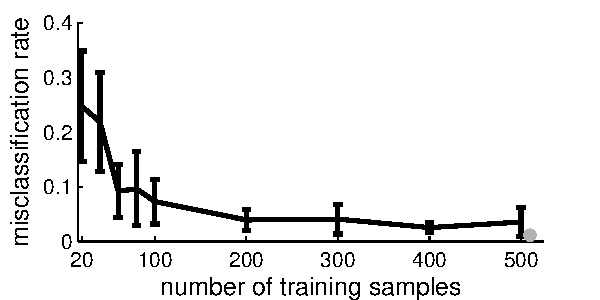
\includegraphics[width=1.0\linewidth]{../figs/hetero_easy_n10_MC5000_QAP_vs_n.pdf}
	\caption{Inexact graph matching can be used to approximate a consistent shuffled graph classifier.  Data in this simulation was sampled from the independent edge model described above.  For each number of training samples, we tested using 5000 test samples, and repeated 10 times.  The gray dot indicates Bayes optimal performance. (NOTE TO CEP: actually, i forgot to QAP the test data to each training class in this example.  i think it would converge much ``faster'' if i included that step. that is, faster in $s$, but now testing requires performing 2 QAPs, whereas before, it did not, so it might actually take longer.  we will see soon, as i'm running that now.)}
	\label{fig:1}
\end{figure}


% section simulated_experiment (end)


\section{Unlabeled Connectome Classification} % (fold)
\label{sub:connectome_classification}

Inspired by the simulated performance of our unlabeled graph classifier, we decided to try it on a real-world application.  A ``connectome'' is a graph in which vertices correspond to biological neural nodes, and edges correspond to connections between the nodes.  Diffusion Magnetic Resonance (MR) Imaging and related technologies are making the acquisition of MR connectomes routine \cite{Hagmann2010}.  49 subjects from the Baltimore Longitudinal Study on Aging comprise this data, with acquisition and connectome inference details as reported in \cite{Gray11}.  Each connectome yields a $70 \times 70$ element binary adjacency matrix.  Associated with each graph is class label based on the gender of the individual (24 males, 25 females).  Because the vertices are labeled, we can compare the results of having the labels and not having the labels.  A $k_n$ nearest neighbor ($k$nn) classifier is universally consistent, that is, guaranteed to achieve optimal performance in the limit \cite{Stone1977}, and therefore seems more appropriate than an independent edge model.  Performance is evaluated with leave-one-out misclassification rate and reported in Table \ref{tab:connectome}. When using the vertex labels, a standard $k$nn achieves $20\%$ misclassification rate.  Chance performance (only using the estimated prior) on this data is $49\%$.  These two numbers provide bounds on performance.  When all graphs are passed through a shuffle channel, we first try to unshuffle the graphs using the above mentioned QAP algorithm.  Given the unshuffled graphs, performance changes to $45\%$, not particularly impressive.  The performance of the independent edge model based Bayes plugin classifier for unlabeled graphs is similarly unimpressive.  We therefore develop a hybrid approach in which the independent edge model is assumed, and parameters are estimated using the vertex labels.  Given these estimates, we can use the QAP algorithm to match each test graph to the two likelihood matrices, and then use the Bayes plugin classifier.  This approach yields a $31\%$ misclassification rate. In contrast, a ``standard'' graph invariant based approach, which computes the graph invariants from \cite{PCP10}, and plugs them into various machine learning algorithms (including the winner \cite{Crammer2008}), yields misclassification rates as low as $25\%$. 


% 
% \begin{itemize}
% 	\item \textbf{Graph Classifier} A Bayes plugin graph classifier as described in \cite{VP11a}, that is, using the labels.
% 	\item \textbf{1-QAP} Estimate the parameters using training data \emph{with} vertex labels.  Then, shuffle the test graph, \qap it to each $\mh{\PP}_y$ matrix.  The  estimated the class is $\mh{y}=\argmax_{y \in \mc{Y}}QAP(G,\mh{\PP}_y)$.   
% 	\item \textbf{48-QAP} Permuting the vertex labels, then implement \texttt{$1$NN$\circ$\qapa}.
% 	% \item \textbf{AVG-QAP}  Permuting the vertex labels, \qapa each of the 48 training graphs to the test graph.  Then, given those permuted adjacency matrices, compute the average, and then implement a standard $1$NN classifier.
% 	\item \textbf{1NN-GI} Use the graph invariant approach as described above. We provide the normalized graph invariants as inputs into a number of standard classifiers, including $k$NN, linear classifiers, support vector machines, random forests, and CW. On this data, the CW classifier performed best; we therefore only report its results.
% \end{itemize}
% 

\begin{table}[h!]
\caption{MR Connectome Leave-One-Out Misclassification Rates}
\begin{center}
\begin{tabular}{|r|r|r|r|r|}
\hline
\texttt{N/A-QAP} & \texttt{1-QAP} & \texttt{48-QAP} & \texttt{1NN-GI}\\
\hline
$20\%$ & $31\%$ & $45\%$  & $25\%$ \\
    \hline
\end{tabular}
\end{center}
\label{tab:connectome}
\end{table}%


\section{Discussion}

In this work, we have address both the theoretical and practical limitations of classifying graphs with and without including labels.  Specifically, we show that shuffling the vertex labels results in an irretrievable situation, with a possible degradation of classification performance, and a necessary degradation if the vertex labels contained class-conditional signal.  Moreover, although one cannot hope to recover the vertex labels, estimating them yields an asymptotically optimal classifier.  This suggest that efforts to estimate the vertex labels may yield useful classification results, outperforming ``standard'' graph-invariant based classifiers.  Via simulation we show that an approximate graph matching algorithm converges to the optimal performance with only about 500 training samples for a particular independent edge random graph model.   Finally, we demonstrate with connectome data that estimating the vertex labels can be useful, but that there remains room to grow to exceed misclassification performance of a carefully chosen graph invariant $\circ$ machine learning based approach on this data.   These connectome data, much like other collections of graphs, can also be equipped with both vertex and edge attributes.  As such, we hope to extend the results herein to consider the more general cases.








% use section* for acknowledgement
\ifCLASSOPTIONcompsoc
  % The Computer Society usually uses the plural form
  \section*{Acknowledgments}
\else
  % regular IEEE prefers the singular form
  \section*{Acknowledgment}
\fi


% Can use something like this to put references on a page
% by themselves when using endfloat and the captionsoff option.
\ifCLASSOPTIONcaptionsoff
  \newpage
\fi


\bibliography{/Users/jovo/Research/latex/library}
\bibliographystyle{IEEEtran}

\begin{IEEEbiography}{Joshua T. Vogelstein}
 is a spritely young man, engorphed in a novel post-buddhist metaphor.

\end{IEEEbiography}


% insert where needed to balance the two columns on the last page with
% biographies
%\newpage


\begin{IEEEbiography}{Carey E. Priebe}
Buddha in training.
\end{IEEEbiography}

% Can be used to pull up biographies so that the bottom of the last one
% is flush with the other column.
% \enlargethispage{-5in}

\end{document}



